% Options for packages loaded elsewhere
\PassOptionsToPackage{unicode}{hyperref}
\PassOptionsToPackage{hyphens}{url}
\PassOptionsToPackage{dvipsnames,svgnames,x11names}{xcolor}
%
\documentclass[
  11pt,
]{article}
\usepackage{amsmath,amssymb}
\usepackage{setspace}
\usepackage{iftex}
\ifPDFTeX
  \usepackage[T1]{fontenc}
  \usepackage[utf8]{inputenc}
  \usepackage{textcomp} % provide euro and other symbols
\else % if luatex or xetex
  \usepackage{unicode-math} % this also loads fontspec
  \defaultfontfeatures{Scale=MatchLowercase}
  \defaultfontfeatures[\rmfamily]{Ligatures=TeX,Scale=1}
\fi
\usepackage{lmodern}
\ifPDFTeX\else
  % xetex/luatex font selection
\fi
% Use upquote if available, for straight quotes in verbatim environments
\IfFileExists{upquote.sty}{\usepackage{upquote}}{}
\IfFileExists{microtype.sty}{% use microtype if available
  \usepackage[]{microtype}
  \UseMicrotypeSet[protrusion]{basicmath} % disable protrusion for tt fonts
}{}
\makeatletter
\@ifundefined{KOMAClassName}{% if non-KOMA class
  \IfFileExists{parskip.sty}{%
    \usepackage{parskip}
  }{% else
    \setlength{\parindent}{0pt}
    \setlength{\parskip}{6pt plus 2pt minus 1pt}}
}{% if KOMA class
  \KOMAoptions{parskip=half}}
\makeatother
\usepackage{xcolor}
\usepackage[margin=1in]{geometry}
\usepackage{longtable,booktabs,array}
\usepackage{calc} % for calculating minipage widths
% Correct order of tables after \paragraph or \subparagraph
\usepackage{etoolbox}
\makeatletter
\patchcmd\longtable{\par}{\if@noskipsec\mbox{}\fi\par}{}{}
\makeatother
% Allow footnotes in longtable head/foot
\IfFileExists{footnotehyper.sty}{\usepackage{footnotehyper}}{\usepackage{footnote}}
\makesavenoteenv{longtable}
\usepackage{graphicx}
\makeatletter
\def\maxwidth{\ifdim\Gin@nat@width>\linewidth\linewidth\else\Gin@nat@width\fi}
\def\maxheight{\ifdim\Gin@nat@height>\textheight\textheight\else\Gin@nat@height\fi}
\makeatother
% Scale images if necessary, so that they will not overflow the page
% margins by default, and it is still possible to overwrite the defaults
% using explicit options in \includegraphics[width, height, ...]{}
\setkeys{Gin}{width=\maxwidth,height=\maxheight,keepaspectratio}
% Set default figure placement to htbp
\makeatletter
\def\fps@figure{htbp}
\makeatother
\ifLuaTeX
  \usepackage{luacolor}
  \usepackage[soul]{lua-ul}
\else
  \usepackage{soul}
\fi
\setlength{\emergencystretch}{3em} % prevent overfull lines
\providecommand{\tightlist}{%
  \setlength{\itemsep}{0pt}\setlength{\parskip}{0pt}}
\setcounter{secnumdepth}{5}
% definitions for citeproc citations
\NewDocumentCommand\citeproctext{}{}
\NewDocumentCommand\citeproc{mm}{%
  \begingroup\def\citeproctext{#2}\cite{#1}\endgroup}
\makeatletter
 % allow citations to break across lines
 \let\@cite@ofmt\@firstofone
 % avoid brackets around text for \cite:
 \def\@biblabel#1{}
 \def\@cite#1#2{{#1\if@tempswa , #2\fi}}
\makeatother
\newlength{\cslhangindent}
\setlength{\cslhangindent}{1.5em}
\newlength{\csllabelwidth}
\setlength{\csllabelwidth}{3em}
\newenvironment{CSLReferences}[2] % #1 hanging-indent, #2 entry-spacing
 {\begin{list}{}{%
  \setlength{\itemindent}{0pt}
  \setlength{\leftmargin}{0pt}
  \setlength{\parsep}{0pt}
  % turn on hanging indent if param 1 is 1
  \ifodd #1
   \setlength{\leftmargin}{\cslhangindent}
   \setlength{\itemindent}{-1\cslhangindent}
  \fi
  % set entry spacing
  \setlength{\itemsep}{#2\baselineskip}}}
 {\end{list}}
\usepackage{calc}
\newcommand{\CSLBlock}[1]{\hfill\break\parbox[t]{\linewidth}{\strut\ignorespaces#1\strut}}
\newcommand{\CSLLeftMargin}[1]{\parbox[t]{\csllabelwidth}{\strut#1\strut}}
\newcommand{\CSLRightInline}[1]{\parbox[t]{\linewidth - \csllabelwidth}{\strut#1\strut}}
\newcommand{\CSLIndent}[1]{\hspace{\cslhangindent}#1}
\usepackage{textcomp}
\usepackage{utopia}
\usepackage{lineno}
\usepackage{float}
\floatplacement{figure}{H}
\usepackage{caption}
\captionsetup[figure]{font=scriptsize}
\captionsetup[table]{font=scriptsize}
\ifLuaTeX
  \usepackage{selnolig}  % disable illegal ligatures
\fi
\usepackage{bookmark}
\IfFileExists{xurl.sty}{\usepackage{xurl}}{} % add URL line breaks if available
\urlstyle{same}
\hypersetup{
  pdftitle={Homo Faber in the making: A cross-cultural analysis of toolmaking skill acquisition in non-industrial societies},
  pdfauthor={Cheng Liu},
  colorlinks=true,
  linkcolor={blue},
  filecolor={Maroon},
  citecolor={Blue},
  urlcolor={Blue},
  pdfcreator={LaTeX via pandoc}}

\title{\emph{Homo Faber} in the making: A cross-cultural analysis of toolmaking skill acquisition in non-industrial societies}
\author{Cheng Liu}
\date{2024-05-10}

\begin{document}
\maketitle

{
\hypersetup{linkcolor=}
\setcounter{tocdepth}{2}
\tableofcontents
}
\setstretch{1.5}
\section{Introduction}\label{introduction}

\subsection{Toolmaking as human experience}\label{toolmaking-as-human-experience}

Toolmaking, together with bipedalism and language, was once regarded as a defining feature that makes humans distinct from other species. Although this notion of human uniqueness was challenged in the past decades by mounting evidence of toolmaking by non-human primates and corvids, it is undoubtedly still critical to human experience in the sense that a biocultural feedback loop is formed through toolmaking that shapes our minds and bodies. Yet the ability to make tools is not born with us, and we all need to either learn from others or through repeated trials and errors. To understand the diversity and universality in the process of human toolmaking skill acquisition, this ongoing project analyzed 169 non-industrial societies displaying varying subsistence strategies around the world using the eHRAF World Cultures database, with a particular focus on developmental contexts and transmission biases involved.

Engaging with the works of Malafouris (\citeproc{ref-ihde2019}{Ihde \& Malafouris, 2019}; \citeproc{ref-malafouris2012}{Malafouris, 2012}) and philosophy of technology (\citeproc{ref-birch2021}{Birch, 2021}; \citeproc{ref-lee2009}{Lee, 2009}).

\subsection{Acquisition of toolmaking skills}\label{acquisition-of-toolmaking-skills}

At the most basic level, this study provides the most in-depth descriptive investigation on this topic so far. It can help improving the external validity of archaeological experimental design. It can serve as a middle-range framework to better understand the formation of archaeological records. Therefore, this paper intends to answer the following three research questions. 1) Do hunter-gatherers have a unique learning pattern compared with groups practicing other types of subsistence strategies? 2) Do learning strategies change across different developmental periods? (More specific hypothesis: will the frequency of social learning decrease through time?) 3) What are some major transmission biases involved? (kin-based? context(success)-based?)

Engaging with the works of Lancy (\citeproc{ref-lancy2017}{Lancy, 2017})

\section{Methods and materials}\label{methods-and-materials}

\begin{enumerate}
\def\labelenumi{\arabic{enumi}.}
\setcounter{enumi}{-1}
\tightlist
\item
  Scope of study: Global sample (\textbf{Figure} \ref{fig:Screeplot})
\end{enumerate}

\begin{figure}

{\centering 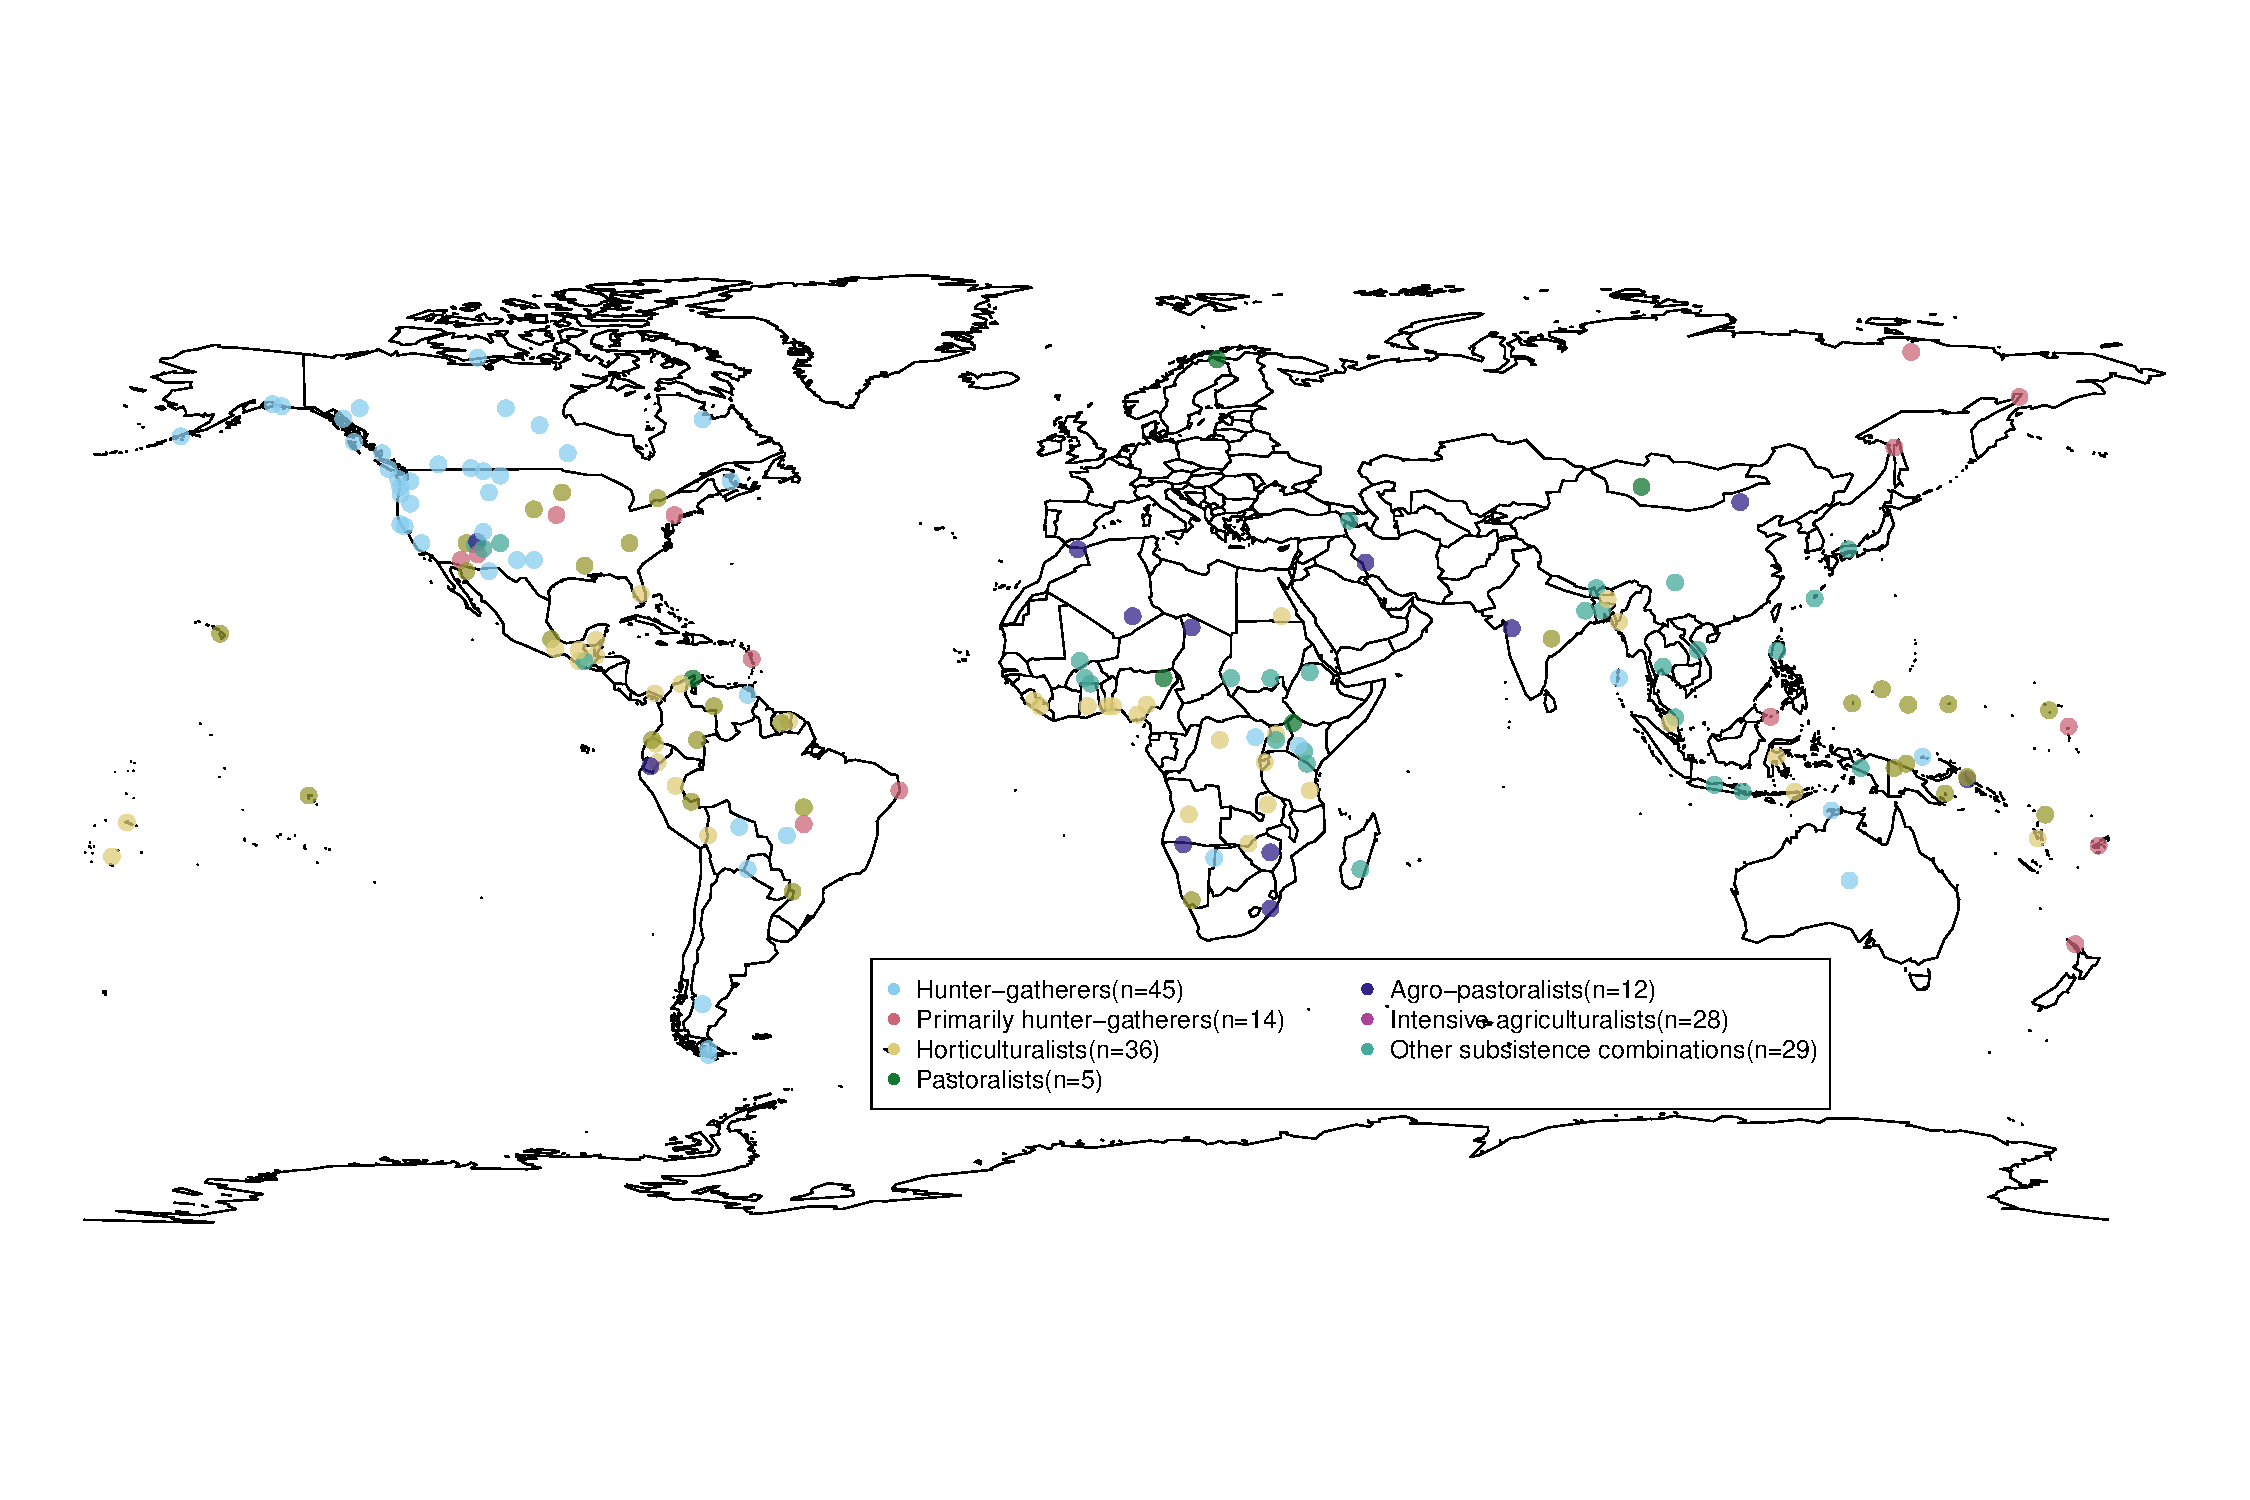
\includegraphics[width=1\linewidth]{../Figure/Fig1} 

}

\caption{The spatial distribution of non-industrial societies covered in this study (n=169). It should be noted that these coordinate data  represent language ‘centroids’ from the open-access language documentation site glottolog.org instead of the real geographical locations of given communities. These language centroids essentially represent the center point of the area where an relevant language is spoken.}\label{fig:Screeplot}
\end{figure}

\begin{enumerate}
\def\labelenumi{\arabic{enumi}.}
\item
  EHRAF World Cultures: subject ``transmission of skills'' + key word ``tool''. This combination yields \st{133 paragraphs in 96 documents across 72 cultures}. Another keywords include \st{make (983 paragraphs in 463 documents across 208 cultures)/made (757 paragraphs in 417 documents across 203 cultures)/making (476 paragraphs in 296 documents across 169 cultures)}, \st{produce (77 paragraphs in 65 documents across 55 cultures)/producing (30 paragraphs in 25 documents across 24 cultures )}, \st{manufacture (59 paragraphs in 48 documents across 43 cultures)/ manufacturing (5 paragraphs in 5 documents across 5 cultures)}, \st{create (39 paragraphs in 33 documents across 30 cultures)/ creating (8 paragraphs in 8 documents across 8 cultures)}, \st{construct (16 paragraphs in 14 documents across 12 cultures)/ constructing (21 paragraphs in 20 documents across 19 cultures )}, \st{assemble (11 paragraphs in 11 documents across 11 cultures)/ assembling (2 paragraphs in 2 documents across 2 cultures)}, \st{fabricate (3 paragraphs in 3 documents across 3 cultures)/ fabricating (1 paragraphs in 1 documents across 1 cultures)}, \st{shape (71 paragraphs in 58 documents across 50 cultures)/ shaping (18 paragraphs in 17 documents across 17 cultures)}, \st{forge (6 paragraphs in 11 documents across 9 cultures)/ forging (6 paragraphs in 6 documents across 5 cultures)}, \st{form (324 paragraphs in 198 documents across 133 cultures)/ forming (15 paragraphs in 15 documents across 14 cultures)}.
\item
  Exclusion criteria: cases of tool use, commercial economy, instance where local people taught the ethnographer how to make tools, instances where it was clearly stated a new form of government-initiated school to save a certain craft, instances where individuals are taught how to make Christianity-related artifacts such altar, and instances where indigenous people mentioned that they learn a specific craft from museum pieces, photographs. However, they may appear as contextual information in the appendix to provide more details of the technologies themselves. archaeological and historical literatures are also excluded.
\end{enumerate}

Variables

\emph{Important Note: ``NA'' is used in all variables when there is not enough information to make the relevant inference, which is different from absence.}

\begin{enumerate}
\def\labelenumi{\arabic{enumi}.}
\item
  \textbf{Area}: using eHRAF's classification system
\item
  \textbf{Society}: using eHRAF's classification system
\item
  \textbf{OWC Code}: The Outline of World Cultures (OWC) is a classification system of the cultures of the world, which is used by eHRAF to organize its databases.
\item
  \textbf{Subsistence}: This variable follows eHRAF's classification system, including Hunter-gatherer, primarily hunter-gatherer, horticulturalist, agro-pastarolist, intensive agriculturalist, other subsistence combinations. The category of commercial economy is excluded.
\item
  \textbf{Year of observation}: The years when the given society was observed by the ethnographers. This information is readily available under the name ``field date'' in the meta information of eHRAF World Cultures.
\item
  \textbf{Location}: The location where the learning event happens according to the ethnographer's description.
\item
  \textbf{Location (type)}: \ul{1) \emph{indoor}}\emph{:} learning happens inside a building; \ul{2) \emph{outdoor settlement}}\emph{:} learning happens inside the settlement but outside the buildings; \ul{3) \emph{outdoor field}}: learning happens outside the settlement
\item
  \textbf{Age of learner}: The learner's age according to the ethnographer's description.
\item
  \textbf{Age group of learner}: \ul{1) \emph{Infancy and Early Childhood}} (0-5 years old), 2\ul{) \emph{Middle Childhood}} (6-12 years old), 3\ul{) \emph{Adolescence}}(13-16 years old), 4\ul{) \emph{Adulthood}} (\textgreater16 years old). For analytical purpose, this category does not concern the cultural differences on the perception of developmental differences. When a age range is provided, the minimal age will be used in the classification of age group.
\item
  \textbf{Number of learner}: The number of learner according to the ethnographer's description.
\item
  \textbf{Age of model}: The model's age according to the ethnographer's description.
\item
  \textbf{Age group of model}: \ul{1) \emph{Infancy and Early Childhood}} (0-5 years old), 2\ul{) \emph{Middle Childhood}} (6-12 years old), 3\ul{) \emph{Adolescence}}(13-16 years old), 4\ul{) \emph{Adulthood}} (\textgreater16 years old).
\item
  \textbf{Number of model}: The number of model according to the ethnographer's description.
\item
  \textbf{Transmission modes}: \ul{1) \emph{horizontal transmission}}: social learning from individuals of the same generation, age group, or cohort, roughly within 4--5 years of age; \ul{2) \emph{vertical transmission}}: children learning from their parents; \ul{3) \emph{oblique transmission}}: social learning between individuals of distinct generations or age groups typically from an older generation to a younger generation. It can happen within or beyond extended kin group, such as learning from grandparents, uncles, or other adults in the local population; \ul{4) \emph{mixed}}: different transmission modes occurred together in the learning process of a given technology.
\item
  \textbf{Social relationship}: The relationship between the learner and the model according to the ethnographer's description. For example, mother-son/father-daughter/etc.
\item
  \textbf{Transmission bias}: This category follows the framework developed by Kendal at al.~(2018). \ul{1) \emph{kin-based bias}}: learning a cultural trait from people who are your kin members, \ul{2) \emph{success-based bias}}: learning a cultural trait from people because they are successful in this technology, \ul{3) \emph{prestige-based bias}}: learning a cultural trait from people because of their high social status; \ul{4) \emph{conformist bias}}: learning a specific type of knowledge from other people because it is displayed by the majority of local population; \ul{5) \emph{mixed}}: different transmission biases occurred together in the learning process of a given technology.
\item
  \textbf{Learning processes}: \ul{1) \emph{individual learning}}: Individual exhibits repeated attempts to learn a skill or develop new skills or knowledge on his or her own, including trial and error and individual practice; \ul{2) \emph{observational learning}}: learner directly observes the actions of models and attempts to replicate the observed actions, and no direct interaction between the model and learner is observed or mentioned; \ul{3) \emph{interactive learning}}: this category features the verbal, gestural and bodily interactions between models and learners, be it formal (``teaching'') or informal (``group play''). It should be noted that these three categories are not mutually exclusive. On the contrary, these three categories are inclusive of each other , where interactive learning is built on both observation and individual practice, and observational learning involves individual practice.
\item
  \textbf{Time spent}: The time spent on learning according to the ethnographer's description.
\item
  \textbf{Time spent (type)}: \ul{1) \emph{one-shot learning}}: the learners only need to learn once to acquire a given technology. \ul{2) \emph{repeated learning}}: the learners need to multiple time, including individual trial-and-error learning and practice, to acquire a given technology.
\item
  \textbf{Technology}: The subject of learning according to the ethnographer's description.
\item
  \textbf{Raw material}: stone, clay, plant, bones, etc.
\item
  \textbf{Restriction of status involved}: The restriction on the social status involved in the learning according to the ethnographer's description. For example, gender, wealth, religious status.
\item
  \textbf{Note} (habit, context, difficulty perceived by local people and ethnographers, access to raw material)
\item
  \textbf{Reference}
\end{enumerate}

\section{Results}\label{results}

\section{Discussion}\label{discussion}

\subsection{Protracted and staged learning trajectories}\label{protracted-and-staged-learning-trajectories}

This study partly confirms Dallos's (\citeproc{ref-dallos2021}{2021}) sharp observation on the significant role of protracted learning in the formation of human culture, as several HRAF ethnographic sources suggested that the learning of toolmaking skills spans multiple developmental periods in an almost structural manner, where each periods feature different approaches to learning and varied task priorities. This applies to scenarios where people learn different different domains of technology at different ages as well as people acquiring one toolmaking skill learn various technological components in a developmentally scaffolding manner. For instance, in Lancy's (\citeproc{ref-lancy1996}{1996}: 161-162) classical ethnography on Kpelle children development, he noted that:

\begin{quote}
``Children learn three types of tasks at three different ages. They begin performing such rudimentary tasks of rice farming as cooking, pounding rice, and chasing away birds at a very early age, usually before they are 9. More difficult tasks, such as hoeing on the farm, net weaving, and trap making, are begun around age 9 and mastered by age 13. Rarer, more complex skills such as cloth weaving, bag weaving, blacksmithing, and medicine making are acquired in the late teens and may be learned after marriage.''
\end{quote}

Canoe making, a skill that demands not only the acquiring of technical know-how but also the development of proper physical strength to handle heavy logs, best illustrates the case of long training period required for a single toolmaking skill. For example, Wilbert (\citeproc{ref-wilbert1976}{1976}: 360) commented that among the Warao hunter-gatherers' skill training for men last until 25 years old and he further(\citeproc{ref-wilbert1977}{Wilbert, 1977}: 23) wrote that:

\begin{quote}
``A boy is associated with canoe-making from early childhood on, initially as spectator, when he accompanies his father and the other men of the family to the forest and watches the production process. Later, as an adolescent, he picks up the axe himself and participates in the process according to his increasing dexterity. By the time he gets married, a young man commands the basic skills and may even have a small canoe to call his own.''
\end{quote}

This pattern of prolonged and staged learning has also recurrently occurred in other ethnographic observations on other indigenous communities such as Chuuk/Truk (\citeproc{ref-goodenough1951}{Goodenough, 1951}: 53-55) in Micronesia, as well as Kapauku (\citeproc{ref-pospisil1958}{Pospisil, 1958}: 40-41) and Trobriands(\citeproc{ref-austen1945}{Austen, 1945}: 194-195; \citeproc{ref-scoditti1989}{Scoditti, 1989}: 56) in Melanesia (e.g., ``15-20 years of apprenticeship''). However, given the inherent constraint that most ethnographic sources used here only provided a fragmented narrative on craft learning, it is still unclear how common is this mode of protracted learning in the manufacturing of smaller-sized tools that does not necessarily require high level of physical strength as debated in several empirical studies regarding humans' unique life history pattern (\citeproc{ref-bliegebird2002}{Bliege Bird \& Bird, 2002}; \citeproc{ref-jones2002}{Jones \& Marlowe, 2002}).

Initiation ceremony is a period for intensive toolmaking skill training, along with other skills required for adulthoold: Laguru, Mende, Eyak, Kaska, Pomo, Maleluka, Tukano, Goajiro, Ona.

\subsection{The distribution of expertise}\label{the-distribution-of-expertise}

\subsection{Co-production as a pedagogy}\label{co-production-as-a-pedagogy}

Kpelle, Garo

\subsection{Skill training: A byproduct of socialization}\label{skill-training-a-byproduct-of-socialization}

\section{Conclusion}\label{conclusion}

People learn most toolmaking skills from their close kins, particularly parents. Extended family members like grandparents and uncles/aunts are also heavily involved in this process. 2) For many skills, they started the learning processes in middle childhood (6-12 years old), which can last for several years. The initiation ceremonies provide opportunities for a period of intensive training. 3) Although individual practice and trial and error always exist, toolmaking skill acquisition involves lots of social interactions, during which causal knowledge is rarely explicitly transmitted.I see it as a stepping stone instead of a definitive text for a better understanding of the subject matter, which merely serves as a starting point for an open dialogue and a project to be collaborated with future researchers like the ``Play Object Play'' database (\citeproc{ref-riede2023}{Riede et al., 2023}).

\section{Acknowledgement}\label{acknowledgement}

This work was assisted in part by skills learned at the 2022 NSF HRAF Summer Institute for Cross Cultural Anthropological Research (NSF BCS Grant \#2020156 to HRAF). The author would also like to thank Carol Ember, Fiona Jordan, and Sean Roberts for their constructive feedback during the early stages of this project.

\section*{References}\label{references}
\addcontentsline{toc}{section}{References}

\phantomsection\label{refs}
\begin{CSLReferences}{1}{0}
\bibitem[\citeproctext]{ref-austen1945}
Austen, L. (1945). New Guinea: Material Culture.: Native Handicrafts in the Trobriand Islands. \emph{Mankind}, \emph{3}(7), 193--198. \url{https://doi.org/10.1111/j.1835-9310.1945.tb01306.x}

\bibitem[\citeproctext]{ref-birch2021}
Birch, J. (2021). Toolmaking and the evolution of normative cognition. \emph{Biology \& Philosophy}, \emph{36}(1), 4. \url{https://doi.org/10.1007/s10539-020-09777-9}

\bibitem[\citeproctext]{ref-bliegebird2002}
Bliege Bird, R., \& Bird, D. W. (2002). Constraints of knowing or constraints of growing? : Fishing and collecting by the children of mer. \emph{Human Nature (Hawthorne, N.Y.)}, \emph{13}(2), 239--267. \url{https://doi.org/10.1007/s12110-002-1009-2}

\bibitem[\citeproctext]{ref-dallos2021}
Dallos, C. (2021). Is there more to human social learning than enhanced facilitation? Prolonged learning and its impact on culture. \emph{Humanities and Social Sciences Communications}, \emph{8}(1), 1--10. \url{https://doi.org/10.1057/s41599-021-00829-3}

\bibitem[\citeproctext]{ref-goodenough1951}
Goodenough, W. H. (1951). \emph{Property, kin, and community on Truk}. Yale University Press. \url{https://ehrafworldcultures.yale.edu/cultures/or19/documents/001}

\bibitem[\citeproctext]{ref-ihde2019}
Ihde, D., \& Malafouris, L. (2019). Homo faber revisited: Postphenomenology and material engagement theory. \emph{Philosophy \& Technology}, \emph{32}(2), 195--214. \url{https://doi.org/10.1007/s13347-018-0321-7}

\bibitem[\citeproctext]{ref-jones2002}
Jones, N. B., \& Marlowe, F. W. (2002). Selection for delayed maturity: Does it take 20 years to learn to hunt and gather? \emph{Human Nature}, \emph{13}(2), 199--238. \url{https://doi.org/10.1007/s12110-002-1008-3}

\bibitem[\citeproctext]{ref-lancy1996}
Lancy, D. F. (1996). \emph{Playing on the mother-ground: Cultural routines for children's development}. Guilford Press.

\bibitem[\citeproctext]{ref-lancy2017}
Lancy, D. F. (2017). Homo faber juvenalis: A multidisciplinary survey of children as tool makers/users. \emph{Childhood in the Past}, \emph{10}(1), 72--90. \url{https://doi.org/10.1080/17585716.2017.1316010}

\bibitem[\citeproctext]{ref-lee2009}
Lee, K. (2009). \emph{Homo faber: the Unity of the History and Philosophy of Technology} (J. K. B. Olsen, E. Selinger, \& S. Riis, Eds.; pp. 13--39). Palgrave Macmillan UK. \url{https://doi.org/10.1057/9780230227279_2}

\bibitem[\citeproctext]{ref-malafouris2012}
Malafouris, L. (2012). Prosthetic gestures: how the tool shapes the mind. \emph{The Behavioral and Brain Sciences}, \emph{35}(4), 230--231. \url{https://doi.org/10.1017/S0140525X11001919}

\bibitem[\citeproctext]{ref-pospisil1958}
Pospisil, L. (1958). \emph{Kapauku papuans and their law}. Yale University Press.

\bibitem[\citeproctext]{ref-riede2023}
Riede, F., Lew-Levy, S., Johannsen, N. N., Lavi, N., \& Andersen, M. M. (2023). Toys as Teachers: A Cross-Cultural Analysis of Object Use and Enskillment in Hunter{\textendash}Gatherer Societies. \emph{Journal of Archaeological Method and Theory}, \emph{30}(1), 32--63. \url{https://doi.org/10.1007/s10816-022-09593-3}

\bibitem[\citeproctext]{ref-scoditti1989}
Scoditti, G. M. G. (1989). \emph{Kitawa: A Linguistic and Aesthetic Analysis of Visual Art in Melanesia}. Walter de Gruyter.

\bibitem[\citeproctext]{ref-wilbert1976}
Wilbert, J. (1976). \emph{To become a maker of canoes: an essay in Warao enculturation} (J. Wilbert, Ed.; Vol. 37, pp. 303--358). UCLA Latin American Center Publications, University of California. \url{https://ehrafworldcultures.yale.edu/cultures/ss18/documents/021}

\bibitem[\citeproctext]{ref-wilbert1977}
Wilbert, J. (1977). \emph{Navigators of the winter sun} (E. Benson, Ed.; pp. 16--46). Dumbarton Oaks Research Library; Collections, Trustees for Harvard University. \url{https://ehrafworldcultures.yale.edu/cultures/ss18/documents/019}

\end{CSLReferences}

\end{document}
